\chapter*{Guilin, Xingping et Yangshuo\markboth{Guilin, Xingping et Yangshuo}{}}
\section*{24 octobre 2015}
Je quitte la province du Guizhou pour arriver dans le Guangxi. La route est encore bien défoncée quand j'entends un frottement sur la roue arrière : c'est la jante qui est fissurée. \newline
 \newline
\centerline{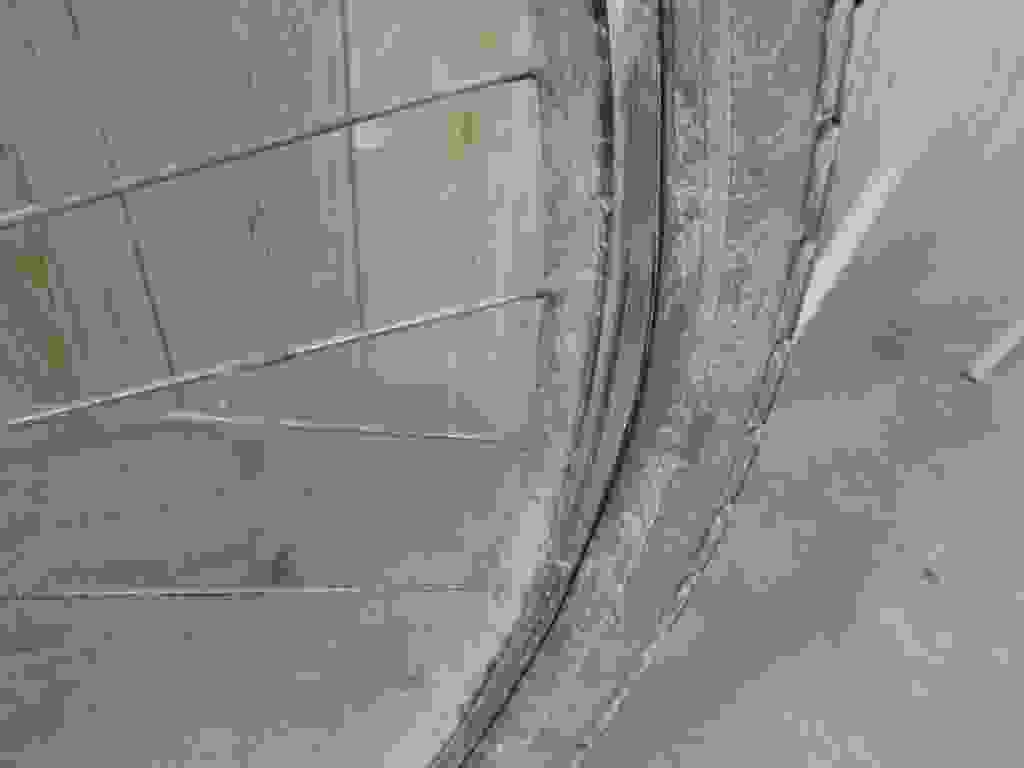
\includegraphics[width=\mywidth]{../wp-content/uploads/2015/10/wpid-oi000027-1024x768.jpg} } 
 \newline
 Ça tient encore 30km jusqu'à la prochaine ville puis je vais à Guilin en bus pour réparer le vélo.  \newline
 Guilin sous le soleil \newline
 \newline
\centerline{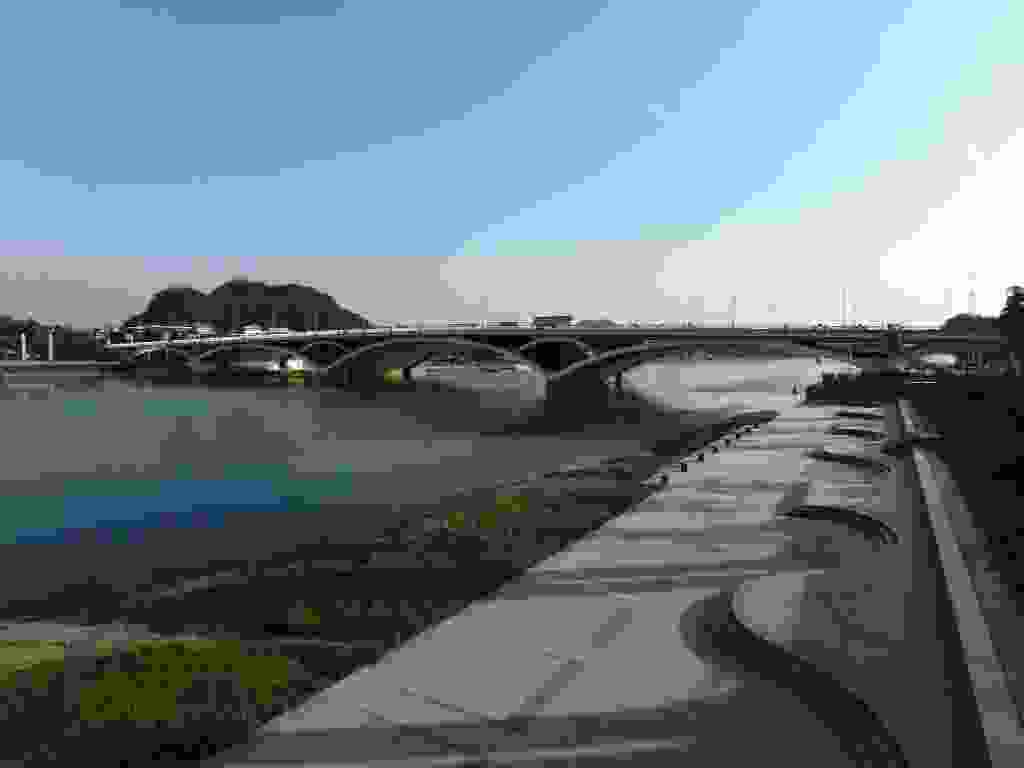
\includegraphics[width=\mywidth]{../wp-content/uploads/2015/10/PA150217-1024x768.jpg} } 
 \newline
 \newline
\centerline{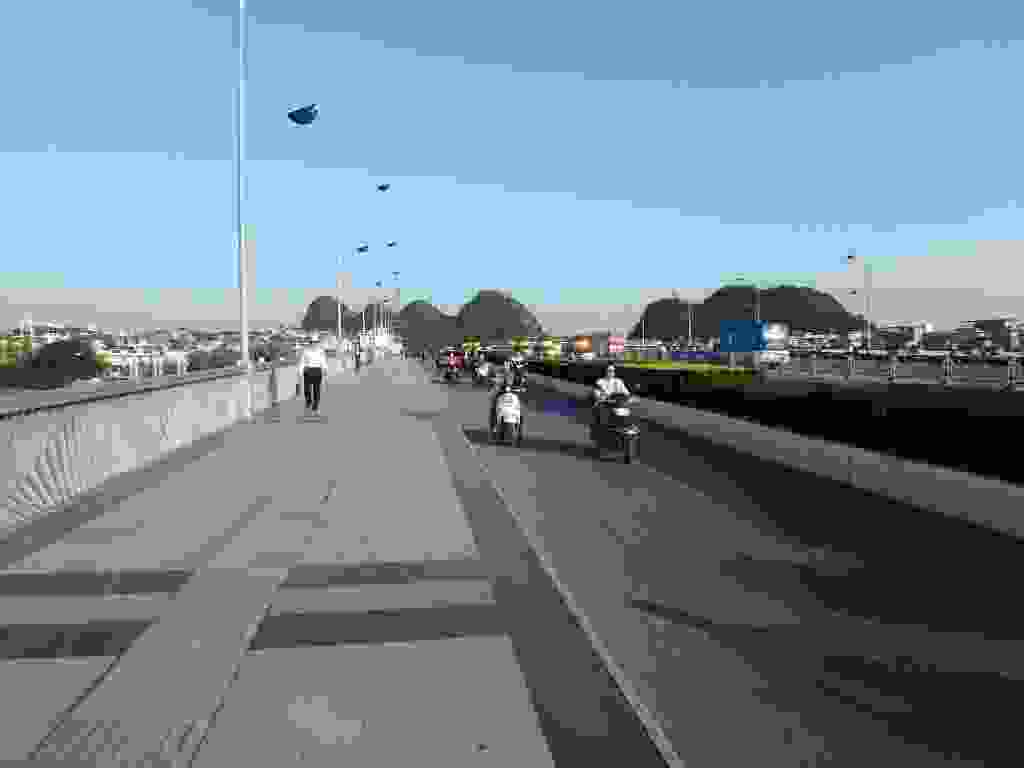
\includegraphics[width=\mywidth]{../wp-content/uploads/2015/10/PA150219-1024x768.jpg} } 
 \newline
 \newline
\centerline{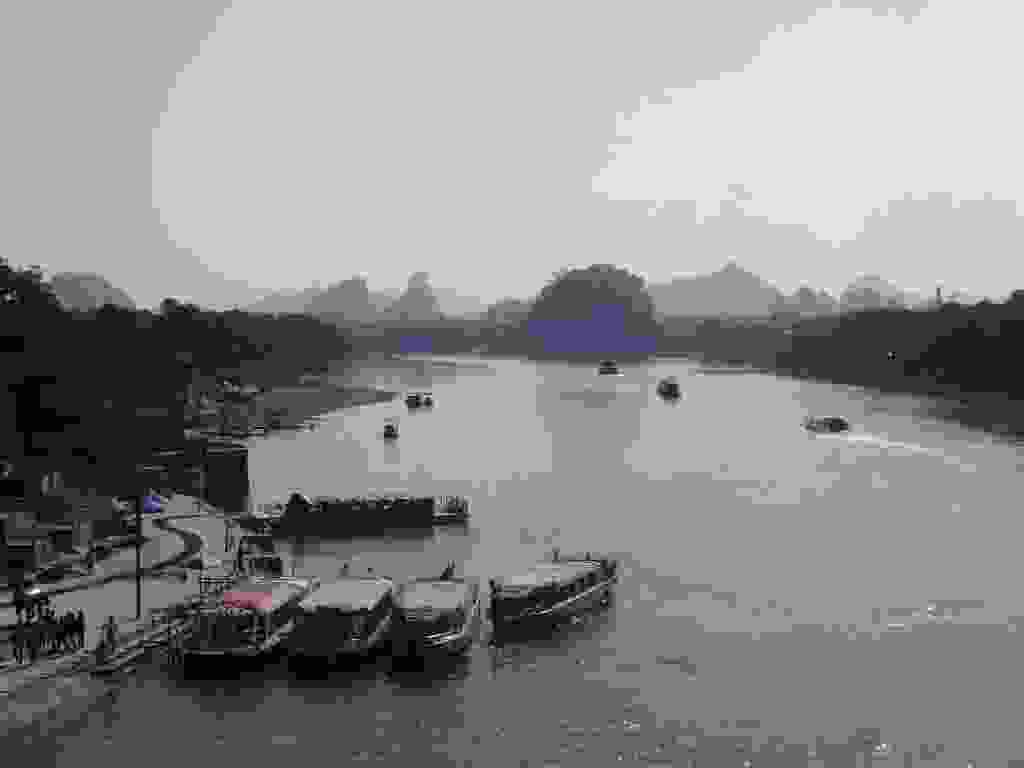
\includegraphics[width=\mywidth]{../wp-content/uploads/2015/10/PA160223-1024x768.jpg} } 
 \newline
 \newline
\centerline{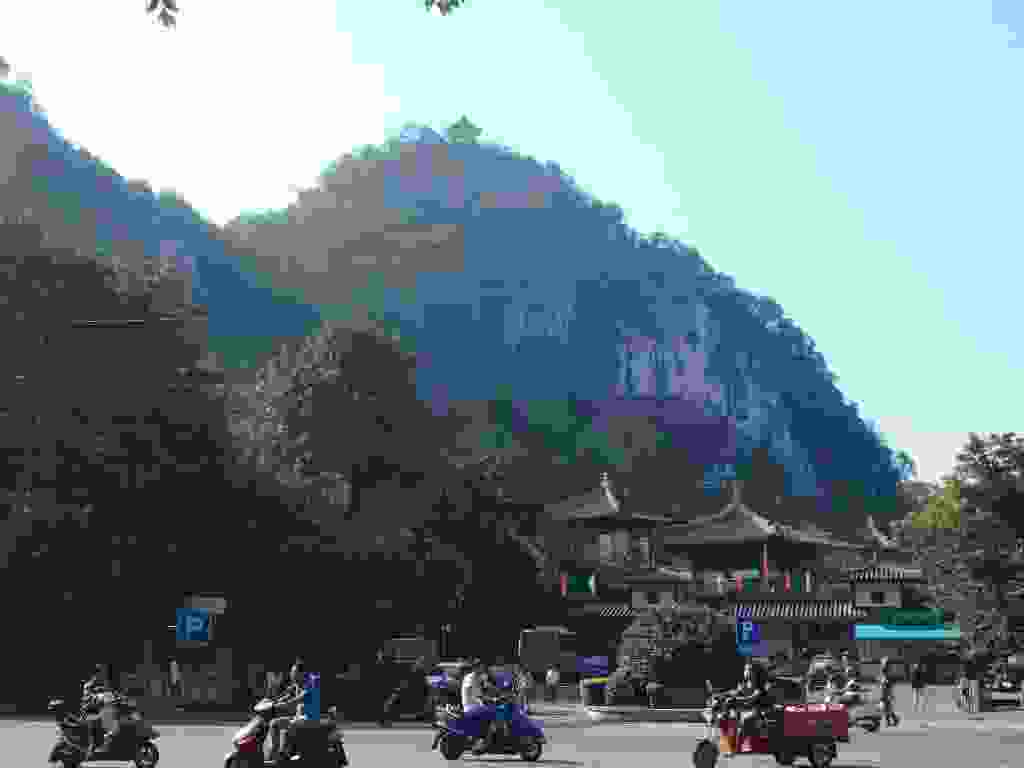
\includegraphics[width=\mywidth]{../wp-content/uploads/2015/10/wpid-oi000028-1024x768.jpg} } 
 \newline
 Pagodes de la Lune et du Soleil \newline
 \newline
\centerline{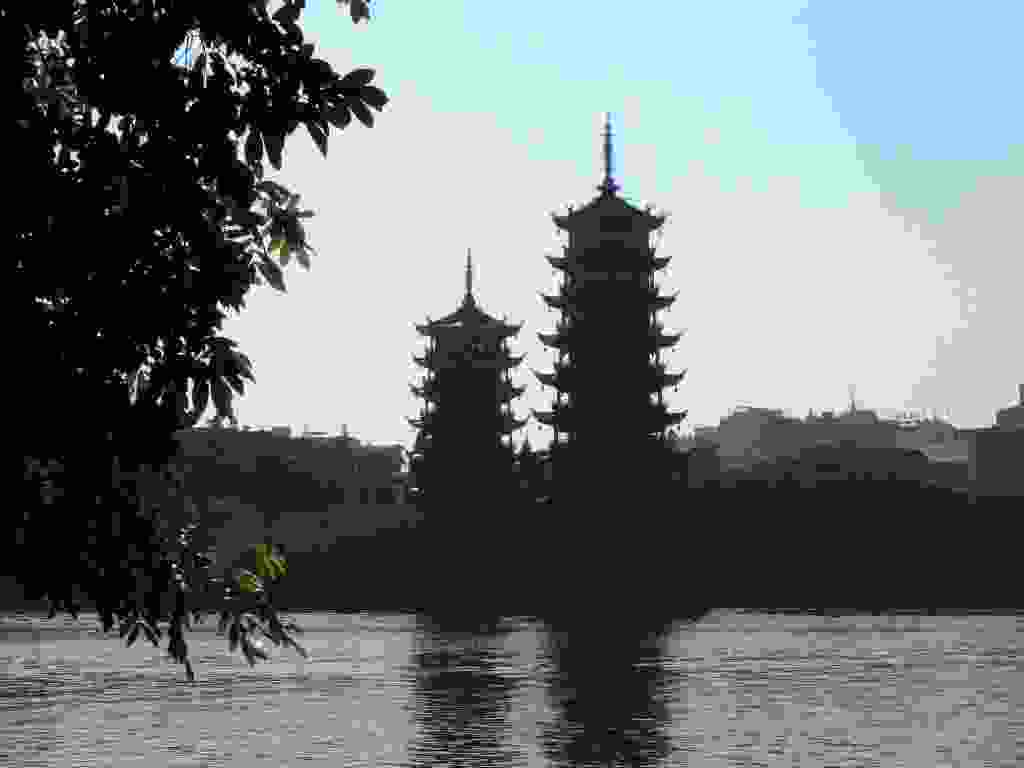
\includegraphics[width=\mywidth]{../wp-content/uploads/2015/10/PA160225-1024x768.jpg} } 
 \newline
 Joueurs de Majong \newline
 \newline
\centerline{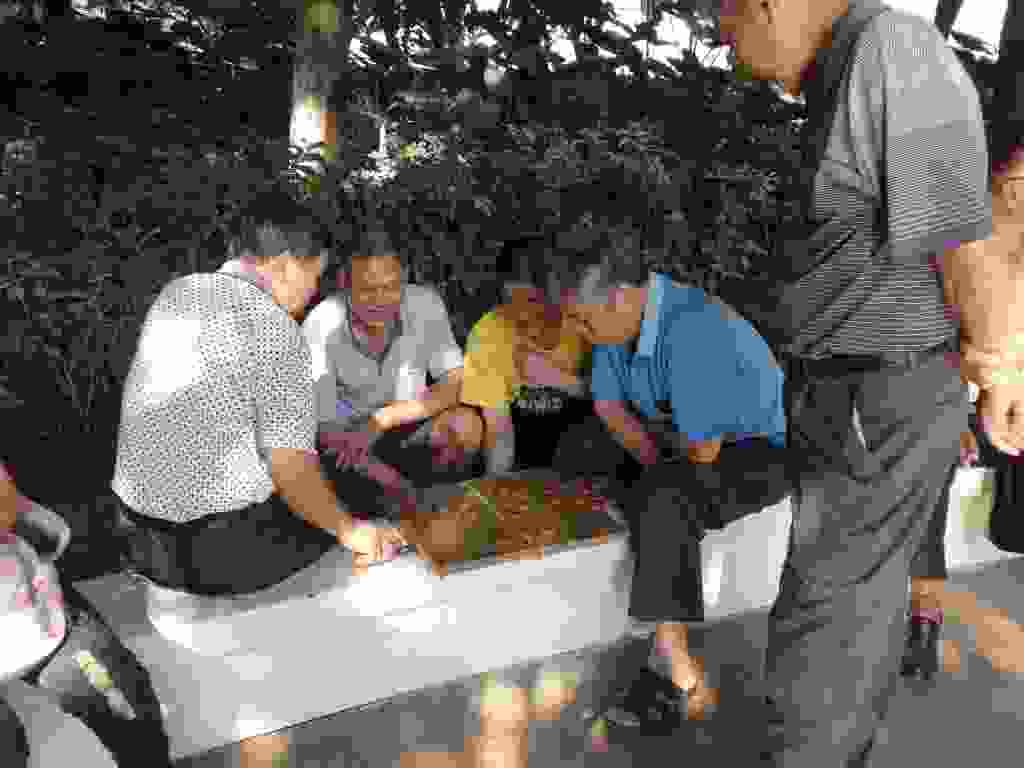
\includegraphics[width=\mywidth]{../wp-content/uploads/2015/10/PA160227-1024x768.jpg} } 
 \newline
 Central square \newline
 \newline
\centerline{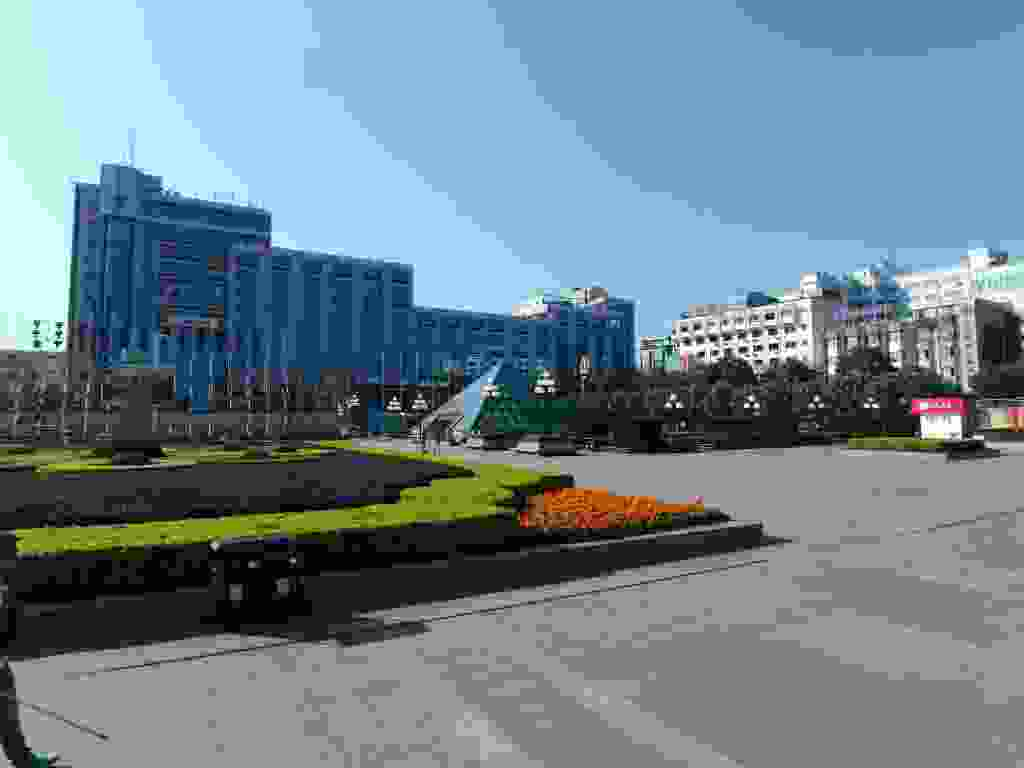
\includegraphics[width=\mywidth]{../wp-content/uploads/2015/10/PA160230-1024x768.jpg} } 
 \newline
 Une fois la roue arrière changée, je pars vers le sud le long de la rivière Li \newline
 \newline
\centerline{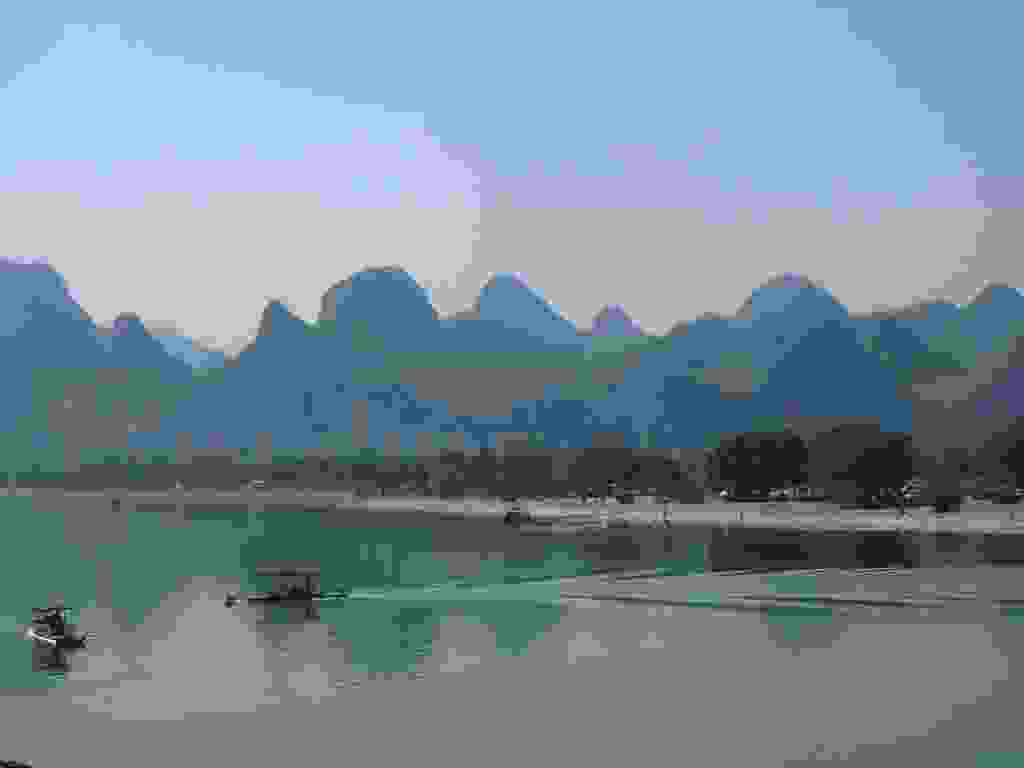
\includegraphics[width=\mywidth]{../wp-content/uploads/2015/10/PA170238-1024x768.jpg} } 
 \newline
 \newline
\centerline{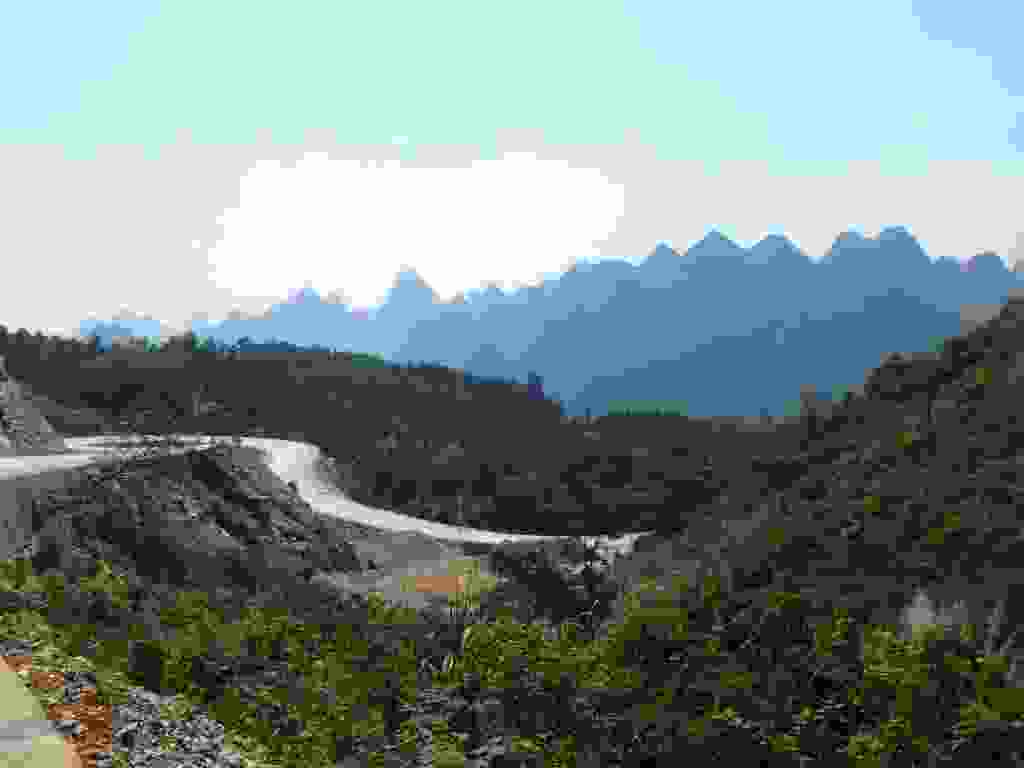
\includegraphics[width=\mywidth]{../wp-content/uploads/2015/10/PA170242-1024x768.jpg} } 
 \newline
 \newline
\centerline{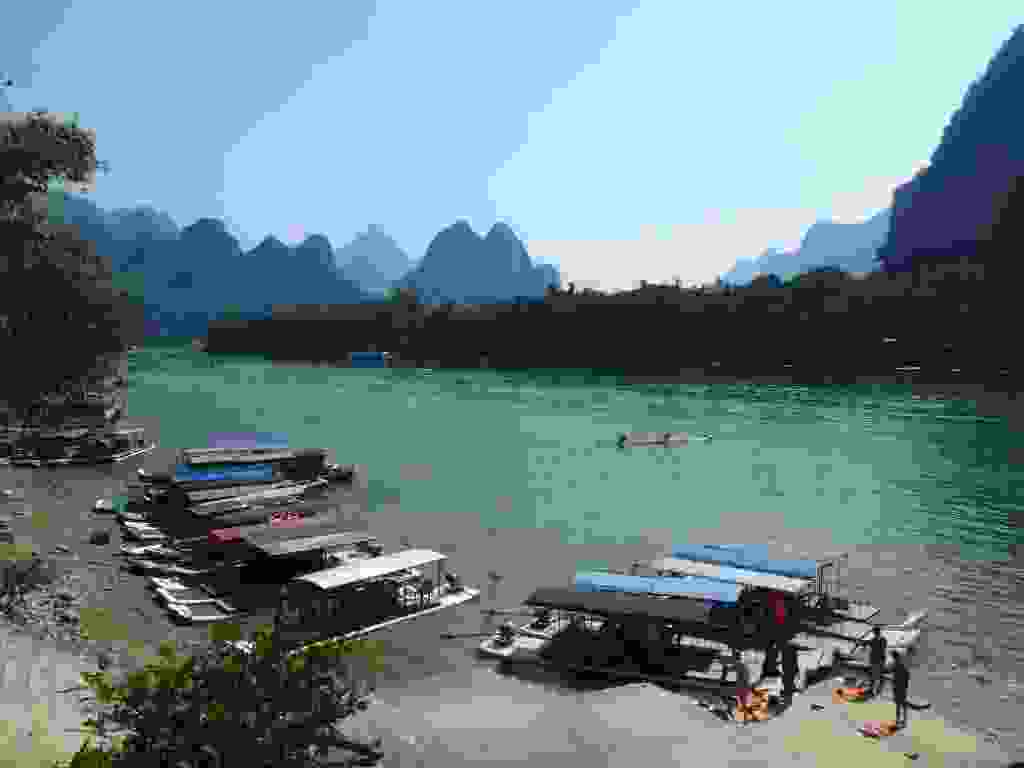
\includegraphics[width=\mywidth]{../wp-content/uploads/2015/10/PA170243-1024x768.jpg} } 
 \newline
 \newline
\centerline{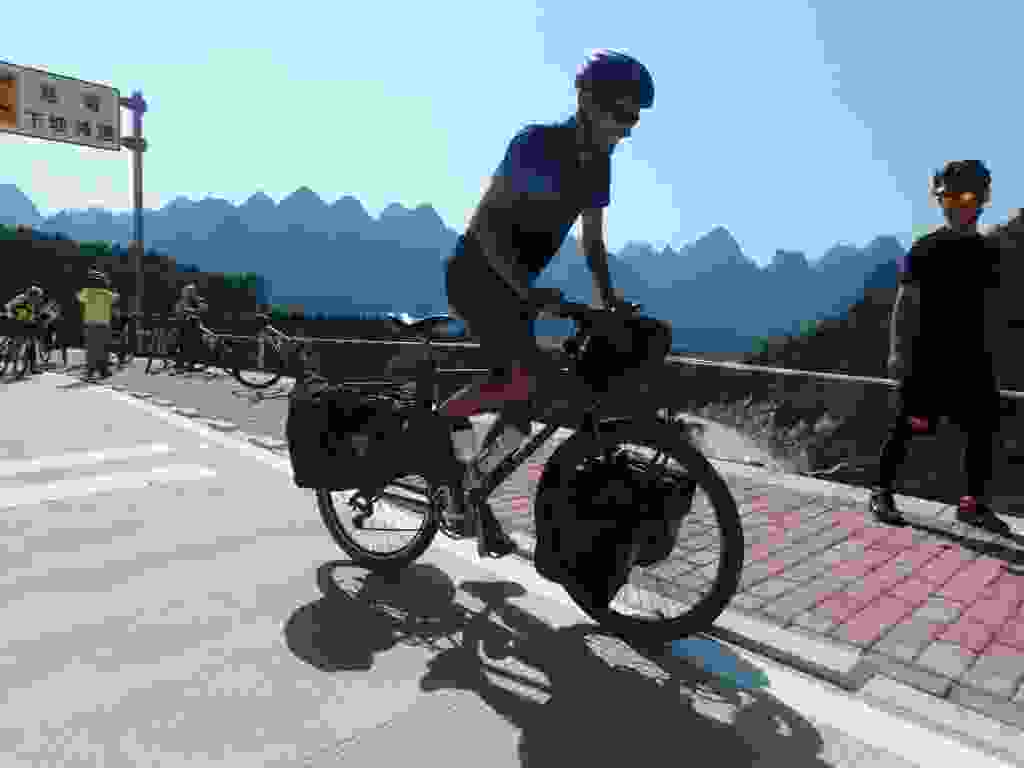
\includegraphics[width=\mywidth]{../wp-content/uploads/2015/10/PA170248-1024x768.jpg} } 
 \newline
 La route s'élève un peu par endroit \newline
 \newline
\centerline{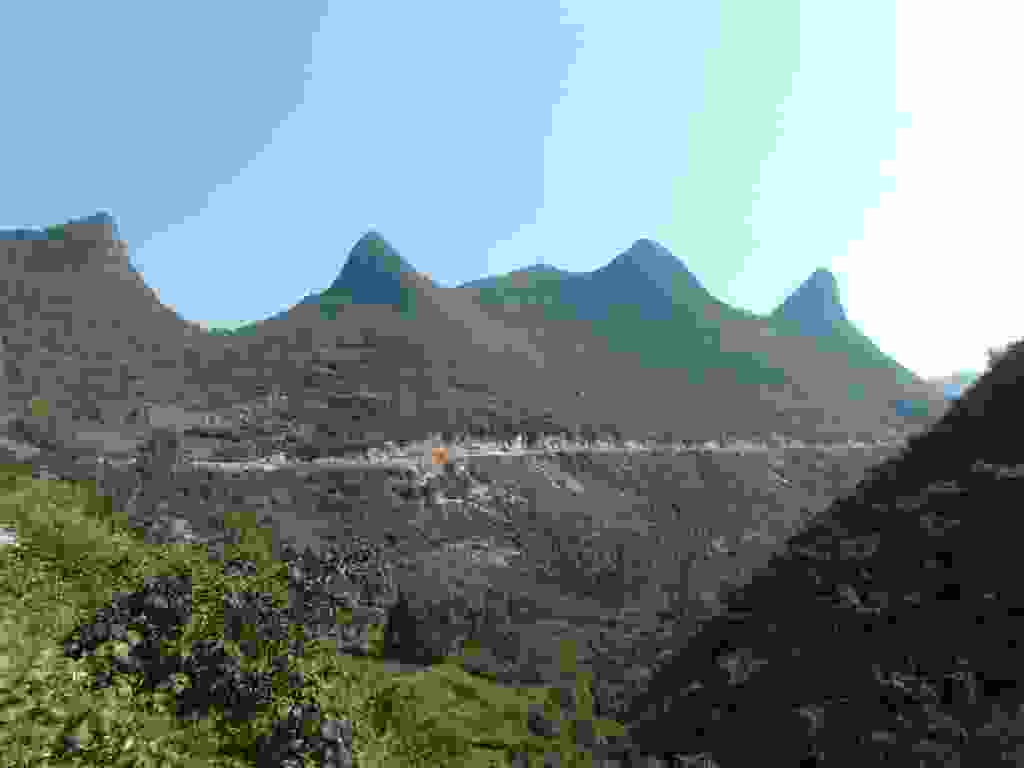
\includegraphics[width=\mywidth]{../wp-content/uploads/2015/10/wpid-oi000030-1024x768.jpg} } 
 \newline
 \newline
\centerline{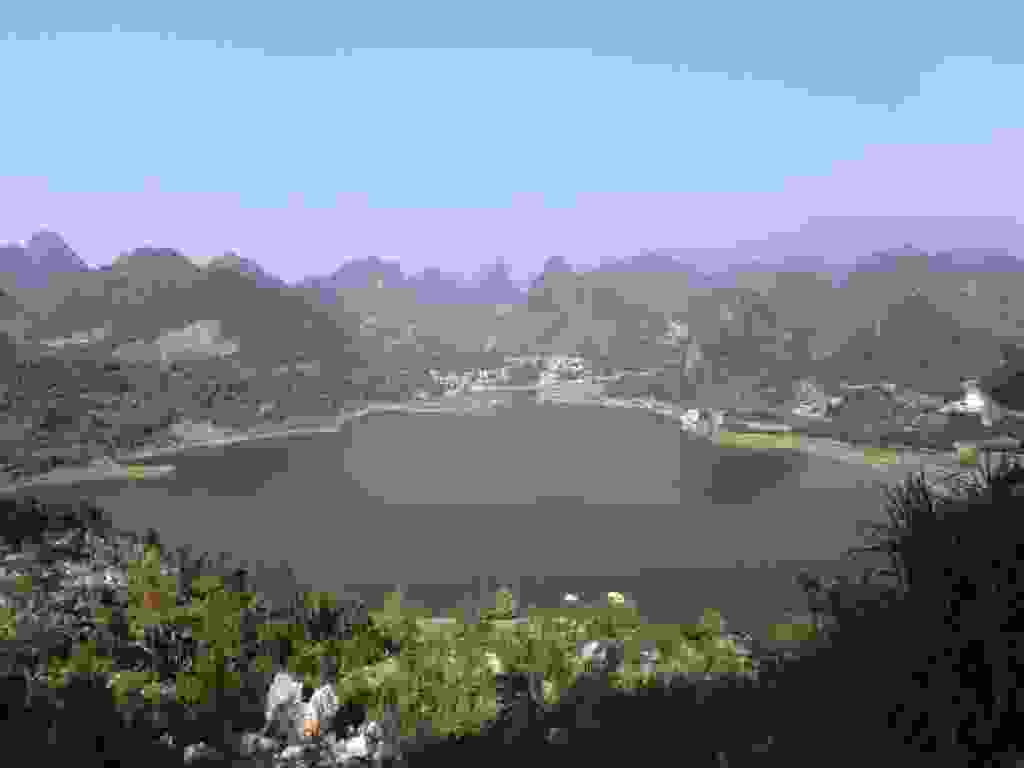
\includegraphics[width=\mywidth]{../wp-content/uploads/2015/10/wpid-oi000032-1024x768.jpg} } 
 \newline
 Je fais étape à Xingping, village touristique au bord de la rivière \newline
 \newline
\centerline{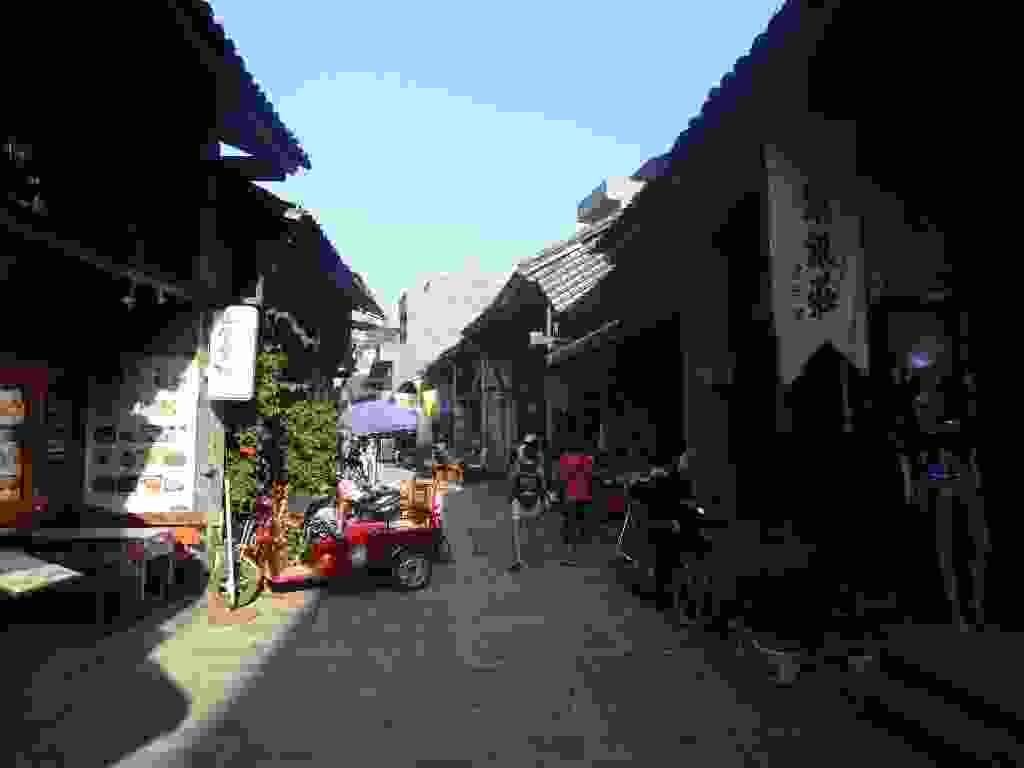
\includegraphics[width=\mywidth]{../wp-content/uploads/2015/10/wpid-oi000033-1024x768.jpg} } 
 \newline
 \newline
\centerline{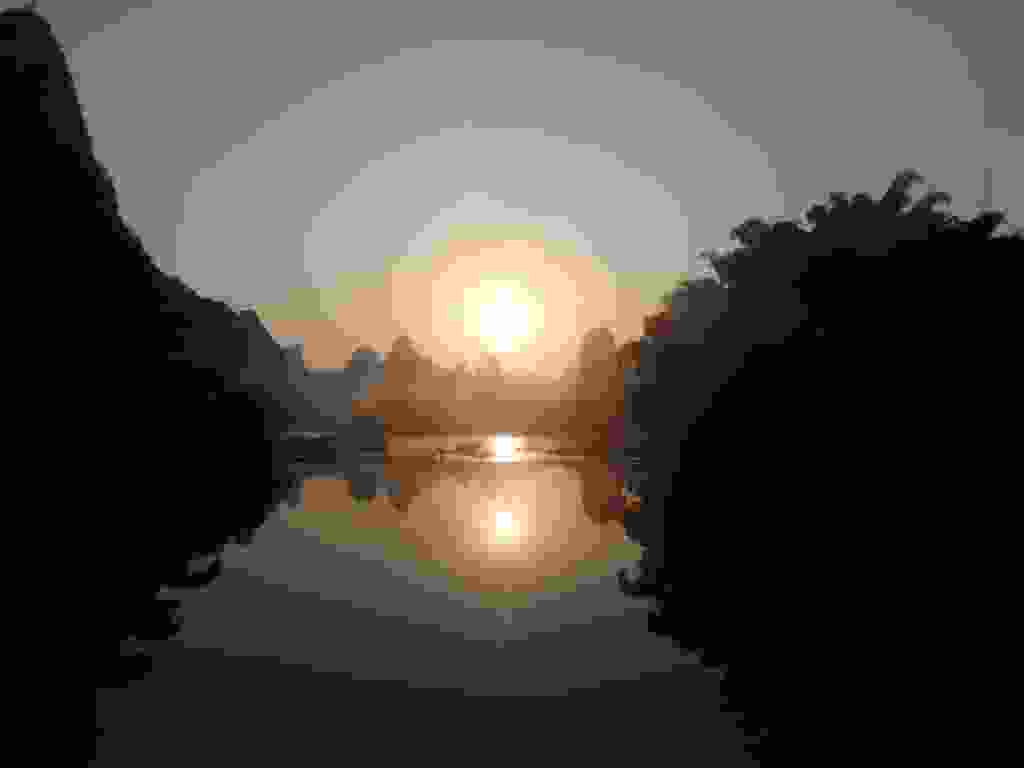
\includegraphics[width=\mywidth]{../wp-content/uploads/2015/10/wpid-oi000034-1024x768.jpg} } 
 \newline
 Coucher de soleil du haut d'une colline \newline
 \newline
\centerline{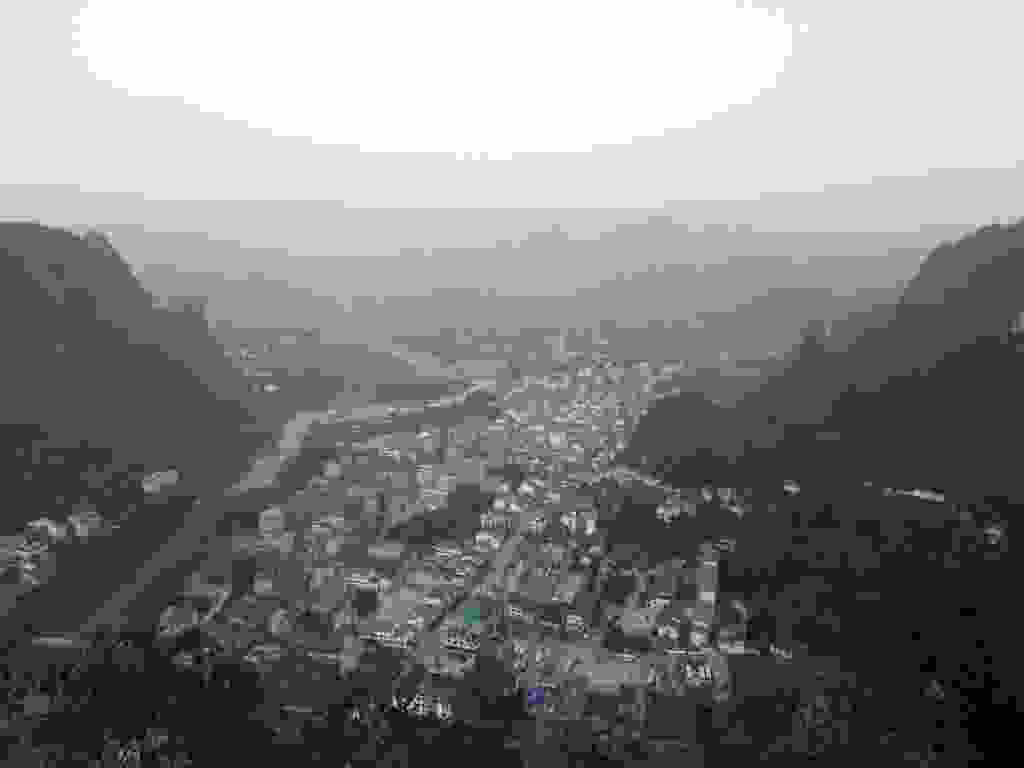
\includegraphics[width=\mywidth]{../wp-content/uploads/2015/10/wpid-oi000035-1024x768.jpg} } 
 \newline
 \newline
\centerline{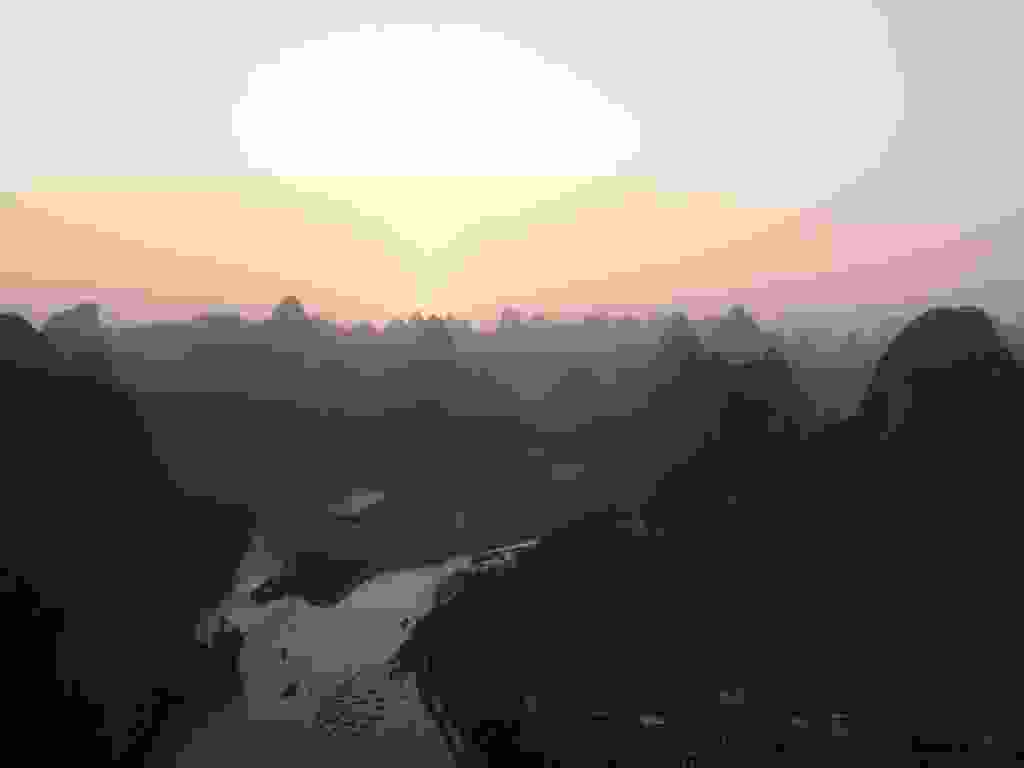
\includegraphics[width=\mywidth]{../wp-content/uploads/2015/10/wpid-oi000036-1024x768.jpg} } 
 \newline
 Célèbre vue sur la rivière Li \newline
 \newline
\centerline{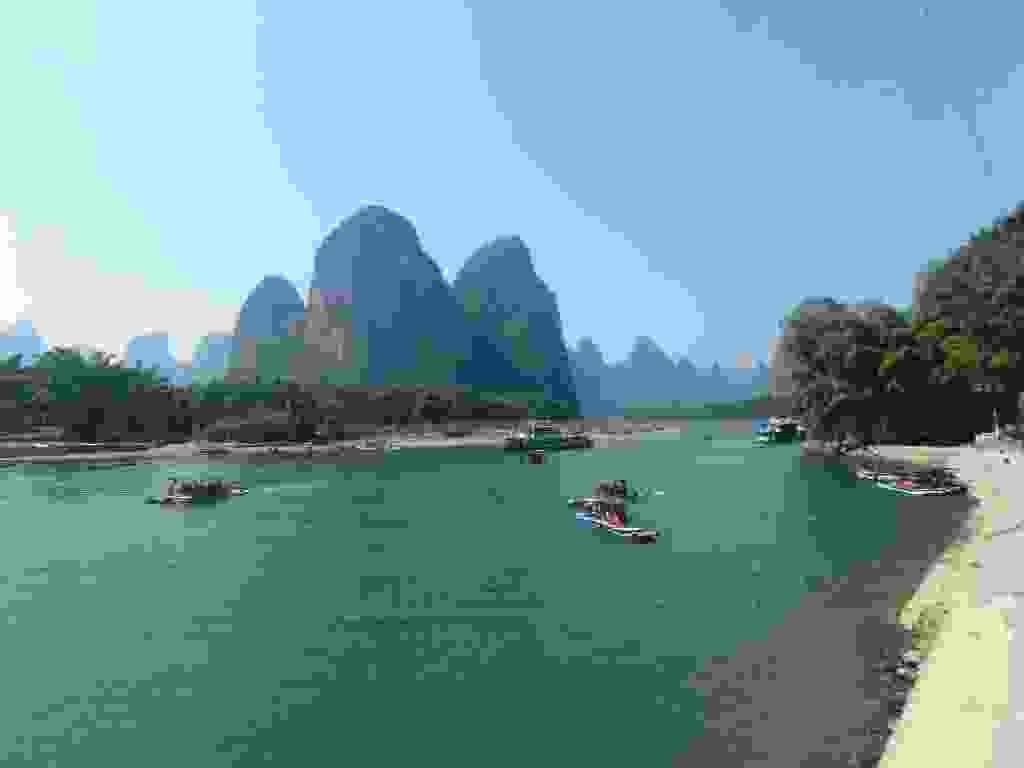
\includegraphics[width=\mywidth]{../wp-content/uploads/2015/10/wpid-oi000037-1024x768.jpg} } 
 \newline
 \newline
\centerline{
\includegraphics[width=\mywidth]{../wp-content/uploads/2015/10/wpid-wp-1445656930044.jpg} } 
 \newline
 Je termine la descente de la rivière à Yangshuo, où je rencontre beaucoup de voyageurs occidentaux : hébergement très bon marché (2.5€ la nuit en dortoir !) et facile pour trouver des pizzas et des burgers \newline
 \newline
\centerline{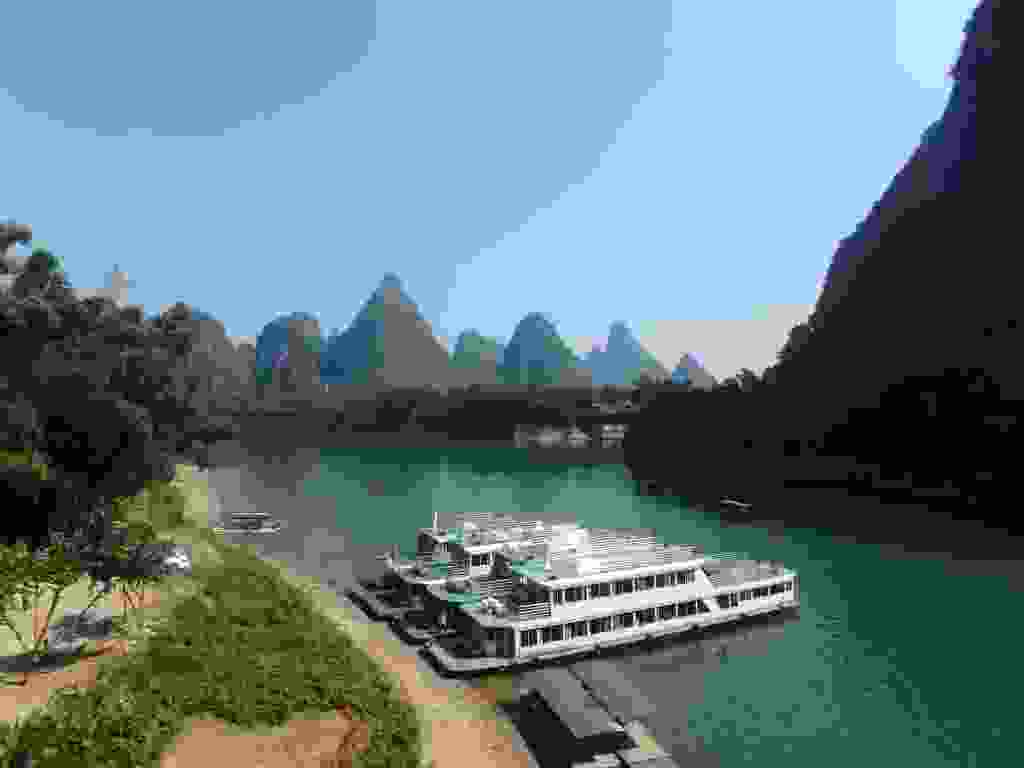
\includegraphics[width=\mywidth]{../wp-content/uploads/2015/10/wpid-oi000039-1024x768.jpg} } 
 \newline
 \newline
\centerline{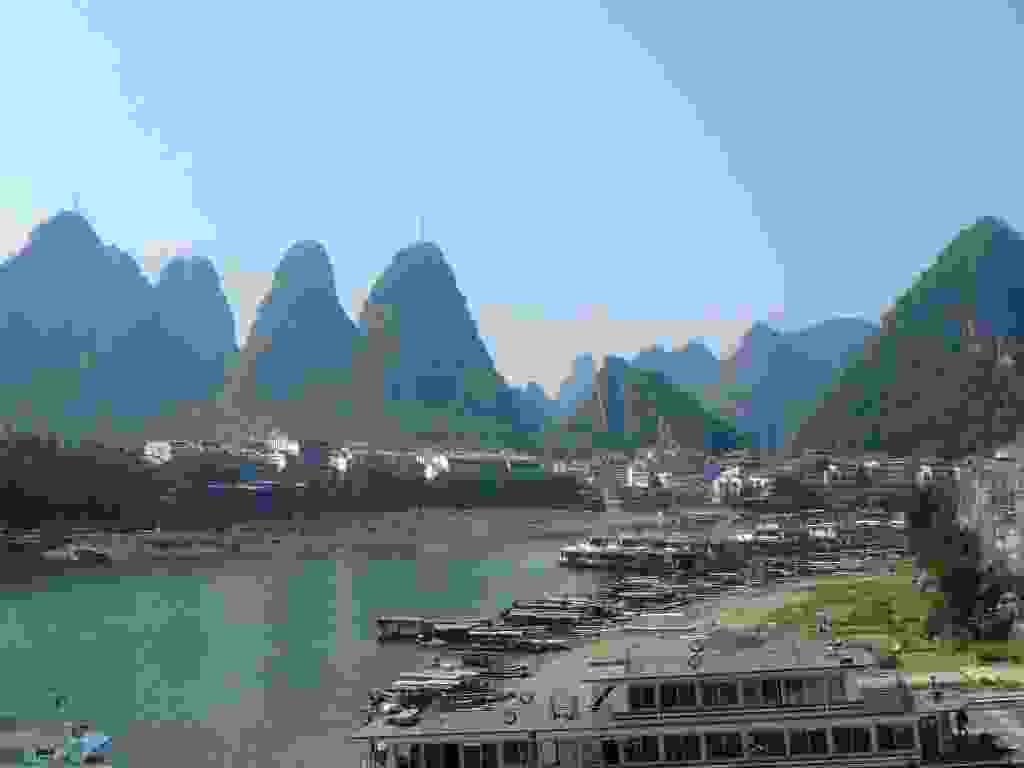
\includegraphics[width=\mywidth]{../wp-content/uploads/2015/10/wpid-oi000038-1024x768.jpg} } 
 \newline
 \newline
\centerline{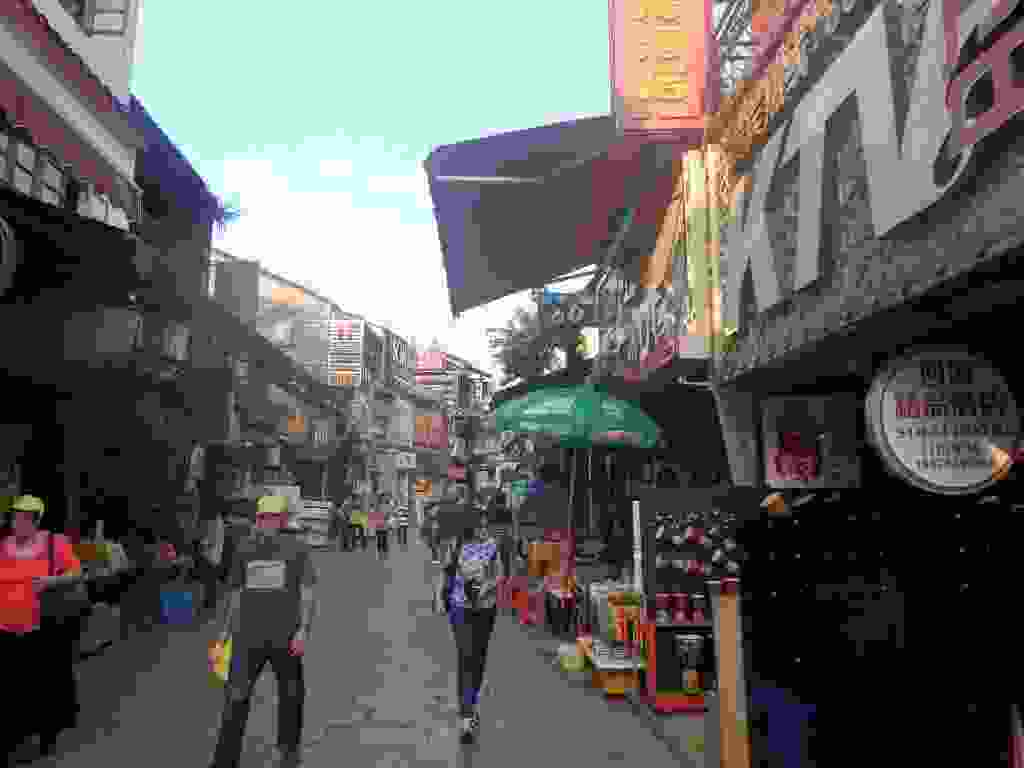
\includegraphics[width=\mywidth]{../wp-content/uploads/2015/10/wpid-oi000040-1024x768.jpg} } 
 \newline
 \newline
\centerline{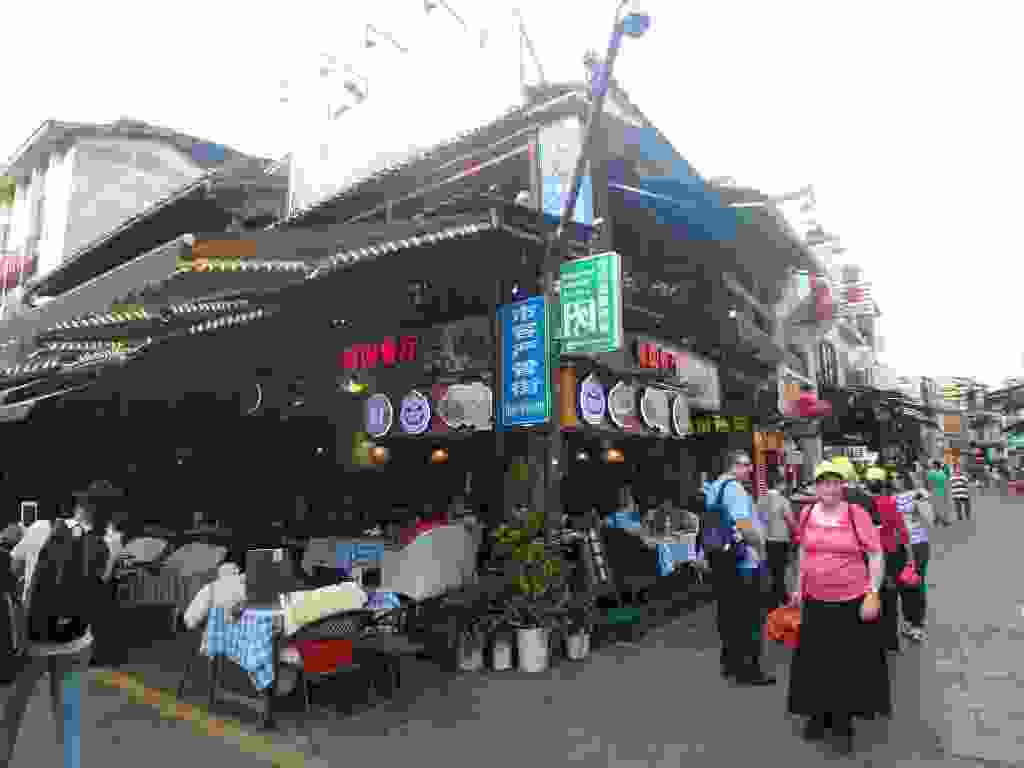
\includegraphics[width=\mywidth]{../wp-content/uploads/2015/10/wpid-oi000041-1024x768.jpg} } 
 \newline
 C'est la dernière étape en Chine, je prends le bus vers Shenzhen où se trouve la frontière avec Hong Kong \newline

\newpage
 
